\documentclass[11pt,a4paper]{article}
\usepackage[utf8]{inputenc}
\usepackage{geometry}
\usepackage[pdftex]{graphicx}
\usepackage{setspace}
\usepackage{natbib}
\usepackage[scaled=0.9]{helvet}
\usepackage{colortbl}
\usepackage{color}
\usepackage{longtable}
\usepackage{rail}

\makeatletter
\def\s@btitle{\relax}
\def\subtitle#1{\gdef\s@btitle{#1}}
\def\@maketitle{%
  \newpage
  \null
  \vskip 2em%
  \begin{center}%
  \let \footnote \thanks
    {\LARGE \@title \par}%
                \if\s@btitle\relax
                \else\typeout{[subtitle]}%
                        \vskip .5pc
                        \begin{large}%
                                \textsl{\s@btitle}%
                                \par
                        \end{large}%
                \fi
    \vskip 1.5em%
    {\large
      \lineskip .5em%
      \begin{tabular}[t]{c}%
        \@author
      \end{tabular}\par}%
    \vskip 1em%
    {\large \@date}%
  \end{center}%
  \par
  \vskip 1.5em}
\makeatother 

\definecolor{gray}{rgb}{0.6,0.6,0.6}
\singlespacing
\oddsidemargin 0in
\headsep 1.3cm
\geometry{left=2cm,top=2cm,right=2cm,bottom=2cm}
\textwidth 17cm
\textheight 24cm
\columnsep 0.0in
\footskip 0.8in


\title{PL/JSON Reference Guide (version 1.0.1)}
\subtitle{For Oracle 10g and 11g}
\author{Jonas Krogsbøll}
\date{}

\railoptions{+ah}
\railalias{quote}{\char"27}
\railalias{dquote}{\char"22}
\railalias{us}{\_}
\railalias{unia}{any Unicode minus ", slash and control chars}
\railalias{unib}{any Unicode minus ', slash and control chars}
\railalias{esc}{escaped character}
\railalias{digits}{0-9}
\railalias{pdigits}{1-9}

\railterm{quote, dquote, us, digits, pdigits}

\begin{document}
\maketitle
\vspace{2in}
\tableofcontents
\newpage

\section{PURPOSE}
The goal of PL/JSON is to create a correct implementation of JSON to use in a PL/SQL environment. The Oracle object syntax has been choosen to ensure a straightforward and easy way to decode and encode JSON. PL/JSON is delivered AS IS and we cannot make any guarantee or be held responsible to any unwanted effects that may arise from using this software. Although we would like to stress that we have tested and used this software and would like to think that is is a safe product to use.

\section{DESCRIPTION}
Parsing and emitting JSON is done in two packages, but you will rarely need to access these directly. The essential objects are linked to the relevant functions in the packages (in constructors and output methods). Basically PL/JSON can be used in two ways: Either you manually build up an object structure and emit JSON text with the to\_char method or you parse JSON text into a object structure and use the objects in PL/SQL. Obvious you could also parse JSON text into objects, modify these and then emit JSON text. There are only three objects you should know: JSON, JSON\_LIST and JSON\_VALUE. The JSON object can hold an object described by the \{ \} syntax and is named JSON rather than JSON\_OBJECT to keep the name short and the fact that an object with the name object sounds silly. The JSON\_LIST object can hold an array described with the [ ] syntax. The postfix "list" was choosen over "array" for two reasons, one: to keep it short, two: there seams to be a naming standard in oracle types that the postfix "array" is being used to describe types with the "table of" construction. The last type JSON\_VALUE contains the primitive simple types (strings, numbers, bools, null), but can also contain an array or an object. The object model for PL/JSON is shown on figure \ref{howjsonwork}.
\begin{figure}[!h]
  \begin{center}
    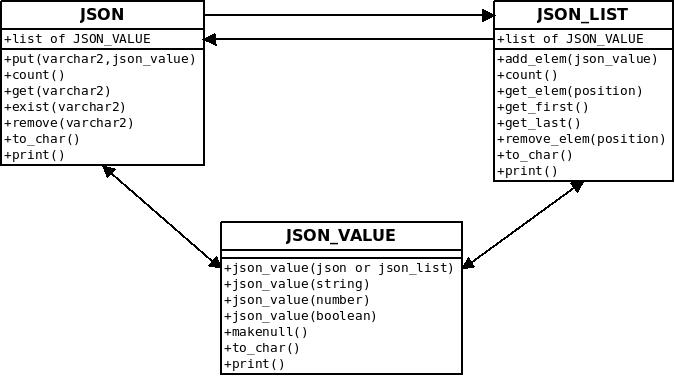
\includegraphics[width=0.8\linewidth]{visual.jpg}
  \end{center} 
  \caption{Essential Objects in PL/JSON}
  \label{howjsonwork}
\end{figure}
\newpage
\section{IN THE RELEASE}
\begin{itemize}
\item Install script
\item Uninstall script.
\item 4 new oracle types ready to use in your database.
\item 3 packages (parser, printer and extension)
\item A few examples files
\item Some testing scripts - creates and delete a table (JSON\_TESTSUITE)
\item Optional addons packages.
\end{itemize}

\section{GETTING STARTED}
To get started using this product, you should first install the product with the install script and then take a look at the examples in the \em examples \em folder. The content of each example file are:
\begin{itemize}
\item \textbf{ex1.sql}: Simple creation of a JSON object. 
\item \textbf{ex2.sql}: Simple creation of a JSON list. 
\item \textbf{ex3.sql}: Working with parser exceptions.
\item \textbf{ex4.sql}: Building an object with the API.
\item \textbf{ex5.sql}: Building a list with the API.
\item \textbf{ex6.sql}: Working with variables as copies.
\item \textbf{ex7.sql}: Using the extension package.
\item \textbf{ex8.sql}: Using JSON Path getters.
\item \textbf{ex9.sql}: Using JSON Path putters.
\item \textbf{ex10.sql}: Using JSON Path remove.
\item \textbf{ex11.sql}: Using the TO\_CLOB method to save JSON.
\item \textbf{ex12.sql}: Pretty print with JSON Path.
\item \textbf{ex13.sql and ex14.sql}: Binary support with base64.
\item \textbf{ex15.sql}: Conversion between JSON and JSON\_LIST.
\item \textbf{ex16.sql}: Dynamic JSON (requires installation of the json\_dyn package).
\item \textbf{ex17.sql}: Duplicate check and fast creation of JSON.
\item \textbf{ex18.sql}: Convert XML to JSON\_LIST with JSONML.
\item \textbf{ex19.sql}: Output unescaped strings.
\end{itemize}
You can also ask questions in the support forum (http://sourceforge.net/projects/pljson/forums/forum/935365) or search the internet for information - google is your friend!

\section{TWEAKS}
You can tweak the behaviour of PL/JSON by setting various variables in the packages. Here comes a description of the possible adjustments you can do. 
\subsection*{JSON\_PRINTER}
In the printer package you can edit the line break method to linux, windows or mac style. You can also change the indentation to the tabular char, or change the number of spaces.

\subsection*{JSON\_PARSER}
The parser is extended to accept more than just pure JSON. The variable "json\_strict" is defaulted to false and can be set to true to force PL/JSON to only accept proper JSON. The current implementation allows input to contain comments with the /* */  notation. Furthermore it extends the definition of a string to allow singlequotes and converts names into strings. The railroad diagram below shows the grammar for names accepted by PL/JSON:
\begin{rail}
name     : (letter) ((letter| digits | us)*);
\end{rail}
However, the values "true", "false" and "null" will not be handled as names.\\
Example of usage with the extended grammar:
\begin{verbatim}
{
  abc : '123"'
}
\end{verbatim}
Parsed and emitted:
\begin{verbatim}
{
  "abc" : "123\""
}
\end{verbatim}

\subsection*{JSON\_PARSER: Javascript functions}
Even though javascript functions are not a part of JSON, you might want to emit functions if your receiving client is a browser. This is how you do it:
\begin{verbatim}
declare
  obj json := json();
begin
  obj.put('test', json_value('function() {return 1;}', esc => false ));
  obj.print;
end;
\end{verbatim}
The output is:
\begin{verbatim}
{
  "test": /**/function() {return 1;}/**/
}
\end{verbatim}
Which is not valid JSON but will work in javascript.\\
The surrounding /**/ is a message to the parser to start and stop building a unescaped json\_value string:
\begin{verbatim}
declare
  obj json := json('{"test": /**/function() {return 1;}/**/}');
begin
  obj.print;
end;
----
{
  "test": /**/function() {return 1;}/**/
}
\end{verbatim}

\subsection*{JSON\_EXT}
The extension package is now mandatory. It contains the path implementation and adds support for dates and binary lob's. Dates is not a part of the JSON standard, so it's up to you to specify how you would like to handle dates. The current implementation specifies a date to be a string that which follows the format: yyyy-mm-dd hh24:mi:ss. If your needs differ from this, then you can rewrite the functions in the package.

\newpage
\section{JSON PATH}
A JSON Path is a way to navigate in a JSON object. The implementation is quite simple and does not support all the features that are available in stefan goessners JavaScript, Python and PHP implementation of JSON Path. Actually, all that is does is to add the support for navigation in JSON, that are allready build in into those languages. When navigating with JSON Path in PL/JSON, members of JSON objects are found with the dot operator while elements in lists are found with square brackets. Accepted input in path navigation is formalized with these railroad diagrams (ws is insignificant whitespace):
\begin{rail}
jsonpath : ((alphanum | 'space')*) \\(( '.' ((alphanum | 'space')+) | '[' ('ws') (string | integer) ('ws') ']' ('ws') )*);
string   : (dquote ((unia|esc)*) dquote) | (quote ((unib|esc)*) quote);
integer  : pdigits (() + digits);
\end{rail}
From version 0.9.6 the implementation accepts an extended grammar where you use a zero-indexed JSON Path.\\
The following examples show how you can use JSON Path to extract from a JSON object.\\\\
The JSON Object:
\begin{verbatim}
{
  "xyz" : {
    "abc" : [1,2,3,[4,5,{"123":45}]]
  }
}
\end{verbatim}
Extract the ''abc'' list:
\begin{verbatim}
json_ext.get_json_list(obj, 
  'xyz.abc').print;
-----------
[1, 2, 3, [4 ,5 , {
  "123" : 45
}]]
\end{verbatim}
Extract the ''123'' number:
\begin{verbatim}
json_ext.get_number(obj,
  'xyz.abc[4][3].123').print;
----------
45
\end{verbatim}
As of version 0.8.4, square brackets can be used to extract JSON members like you would do in JavaScript: 
\begin{verbatim}
json_ext.get_number(obj,
  '["xyz"]["abc"][4][3]["123"]').print;
----------
45
\end{verbatim}
You can also use JSON Path to modify an existing JSON Object:
\begin{verbatim}
json_ext.put(obj, 'xyz.abc',
  json('{"val":123}'));
----------
{
  "xyz" : {
    "abc" : {
      "val" : 123
    }
  }
}
\end{verbatim}
Remove unwanted elements is also an option:
\begin{verbatim}
json_ext.remove(obj, 'xyz.abc');
----------
{
  "xyz" : {
  }
}
\end{verbatim}
In the 0.9.1 release, both JSON and JSON\_LIST are hooked to the JSON Path implementation:
\begin{verbatim}
declare
  v_obj json := json('{a:true}');
  v_list json_list := json_list('[1,2,[3,4]]');
begin
  v_obj.path('a').print;
  v_list.path('[3][1]').print;
end;
----------
true
3
\end{verbatim}
The example files 8 to 10 provides a more detailed explaination.\\
\\
In the 0.9.2 release, it is also possible to use path to modify objects and arrays:
\begin{verbatim}
declare
  v_obj json := json('{a:true}');
  v_list json_list := json_list('[1,2,[3,4]]');
begin
  v_obj.path_put('a[2]', json_list('[true, true]'));
  v_obj.print;
  v_list.path_put('[3][1]', 'test');
  v_list.print;
end;
----------
{
  "a" : [null, [true, true]]
}
[1, 2, ["test", 4]]
\end{verbatim}

\section{BEHAVIOR \& ERROR HANDLING}
Input to the parser is expected to be in the charset of the database. The objects that are generated contains unescaped values that will be escaped when emitted through the printer. To ensure correct JSON output, even from non-UTF databases, only ASCII chars are emitted. All the characters which are not part of ASCII will be escaped. 
\\
The errors or exceptions that PL/JSON may throw, can be catched with the following code:
\begin{verbatim}
declare
  scanner_exception exception;
  pragma exception_init(scanner_exception, -20100);
  parser_exception exception;
  pragma exception_init(parser_exception, -20101);
  jext_exception exception;
  pragma exception_init(jext_exception, -20110);
  ...
begin
  ... json code ...
exception
  when scanner_exception exception then ...
  when parser_exception exception then ...
  when jext_exception exception then ...
end;
\end{verbatim}

\section{KNOWN LIMITATIONS}
\begin{itemize}
\item key-names are limited to 4000 characters.
\item The number parsing assumes that oracles number type can contain the input (in most cases it can).
\end {itemize}

\section{TESTSUITE}
Any proper product is tested for correctness. So should PL/JSON be, with a testsuite that can be executed without installing any additional software on your database. You probaly don't need the testsuite, but if you modify the implementation or add more features, tests will be needed. Also if you discover a bug, you could report the bug by writing a relevant testcase.

\section{CONTRIBUTING}
Write to us in the forums of sourceforge.net. We will be happy to hear from you. \\\\
Q: ''I've added a lot of code, please merge my changes''\\
A: Hmmm - it's not that we don't appriciate your work, but we would really prefer that you wrote tests and documentation to each feature - otherwise new code could easily break functionality. \\\\
Q: ''I've added some changes and I might contribute them to the project, but what's in it for me?''\\
A: This is not GPL, so you can keep your changes if you want to. 
When you are contributing then more eyes will look at your code. 
Possible errors might get detected and corrected and new features may arrise from your features - making it a better product you can use.

\section{OPTIONAL PACKAGES}
\begin{itemize}
\item JSON\_DYN A package that enables you to generate JSON from sql. Nested queries are not supported. See example 16 for more information.
\item JSON\_ML A package that converts from XML to JSON using a XSLT stylesheet. See www.jsonml.org.
\item JSON\_XML A package that converts a JSON object to XML. 
\item JSON\_UTIL\_PKG Written by Morten Braten (http://ora-00001.blogspot.com). Generate JSON from sql using a XSLT stylesheet. 
\end{itemize}

\end{document}



